%!TEX root = ../Thesis.tex
\section{Foundational Research}

The foundational research in this thesis includes publications on \acl{dl} and 4D seismic in \cref{sec:foundations}. These publications apply a signal processing-approach to both 4D seismic and \acl{ml}. I include a paper that takes a tutorial-view of dynamic time-warping a 4D seismic time shift analysis tool and introduces a novel constraint to improve performance of the algorithm. I then go on to present a possible source of misclassification in neural networks on non-stationary physical data like seismics. I further investigate a possible solution to the aliasing problem of \aclp{cnn} for seismic, including complex-valued operations withing the network. I further investigate the assumption that massive interpreted datasets have to be available for successful training of \aclp{dnn} and present a working solution for smaller datasets.

% dramsch2019dtw
\citet{dramsch2019dtw} presents a tutorial of \acf{dtw}. \ac{dtw} is a powerful signal processing tool introduced to 4D seismic analysis by \citep{Hale2013} on synthetic data. 4D seismic data relies on alignment of the seismic volumes. This enables interpreters to compare the amplitudes differences of the data. Due to the capability of \ac{dtw} to match arbitrary time-series, it is applicable to 4D time shifts, seismic-well ties, well-to-well ties, and seismic pre- and post-stack migration \citep{Luo*2014}.  \ac{dtw} is known to be computationally slow and expensive, while extracting poor matches on seismic field data. This tutorial paper goes into detail of the \ac{dtw} algorithm, exploring similarity measures, optimization, and constraints interactively through reproducible implementation in Python.

\begin{algorithm}
\caption{\acl{dtw}} \label{dtw}
\begin{algorithmic}[1]
\State Given: Trace $a$ and Trace $b$ of lengths $n$.
\State Calculate distance matrix $D$
\State $D \gets dist(a,b)$
\State Calculate Cumulative Cost $C$
\State $C[0,0] \gets 0$
\For {$i = 1$ to $n$} \Comment{Populate Edge}
    \State $C[0,i] \gets C[0,i] + C[0,i-1]$
    \State $C[i,0] \gets C[i,0] + C[i-1,0]$
\EndFor
\For {$i = 1$ to $n$} \Comment{Fill Cumulative Cost Matrix}
    \For {$j = 1$ to $n$} 
        \State $C_{min} \gets \textbf{min} \{C[i,j-1], C[i-1,j-1], C[i-1,j]\}$
        \State $C[i,j] \gets C[i,j] + C_{min}$
    \EndFor
\EndFor
\State Backtrack minimum cost path $P$
\State \Return {P}
\end{algorithmic}
\end{algorithm}

The \ac{dtw} algorithm relies on calculating a distance matrix sample-wise between two traces. This is the first avenue of optimization we explore in this paper. The commonly used $L_1$ norm to calculate the distance norm is shown to perform worst out-of-the-box calculating $|b-a|$. Alternatively, the euclidean distance or $L_2$ norm can be used, which modifies the calculation to $(b-a)^2$. The difference between $L_1$ and $L_2$ is significant in the sense that the $L_1$ norm is not differentiable or convex, however it scales linearly for outliers. The $L_2$ norm converges fast close to zero, however the error "explodes" for outliers. We introduce a constraint used in convex optimization, which combines the advantages of the $L_1$ norm and $L_2$ norm, namely the Huber loss:

\begin{equation}
L_\delta (a, b) = 
\begin{cases}
 \frac{1}{2} (b-a)^2 & \text{for } |b-a| \le \delta, \\
 \delta (|b-a| - \frac{1}{2} \delta), & \text{otherwise.}
\end{cases}
\label{eq:huber}
\end{equation}

which is convex for small values, scales linearly for outliers and is differentiable for all values of $\mathbb{R}$, with $\delta$ being a scaling factor.


\begin{figure}[!ht]
    \subbottom[\citet{Itakura1975} Parallelogram]{%
     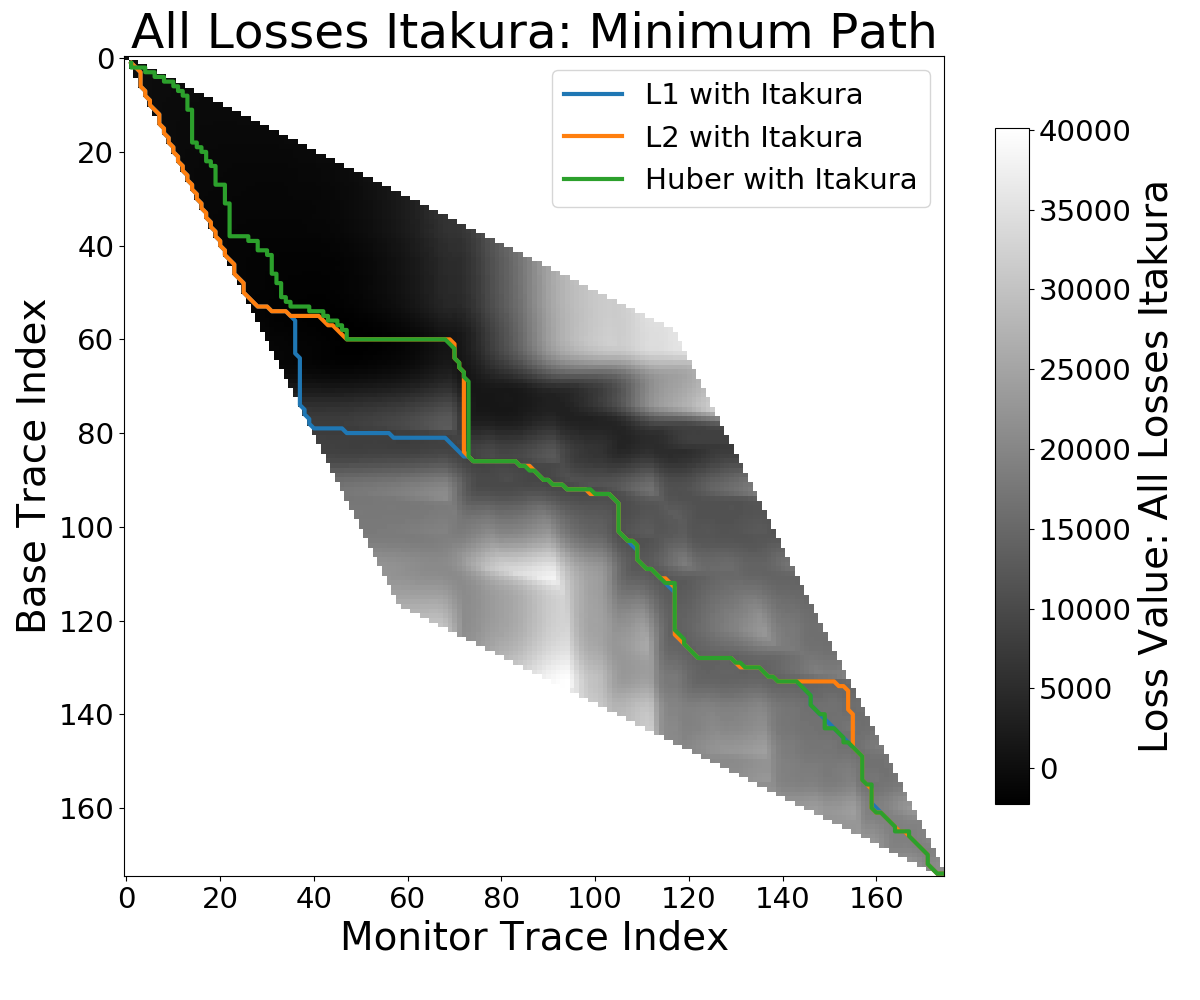
\includegraphics[width=.3\textwidth]{figures/minimum_path_all_losses_itakura_.png} \label{fig:itakura}
    }
    ~
    \subbottom[\citet{Sakoe1978} Disc]{%
     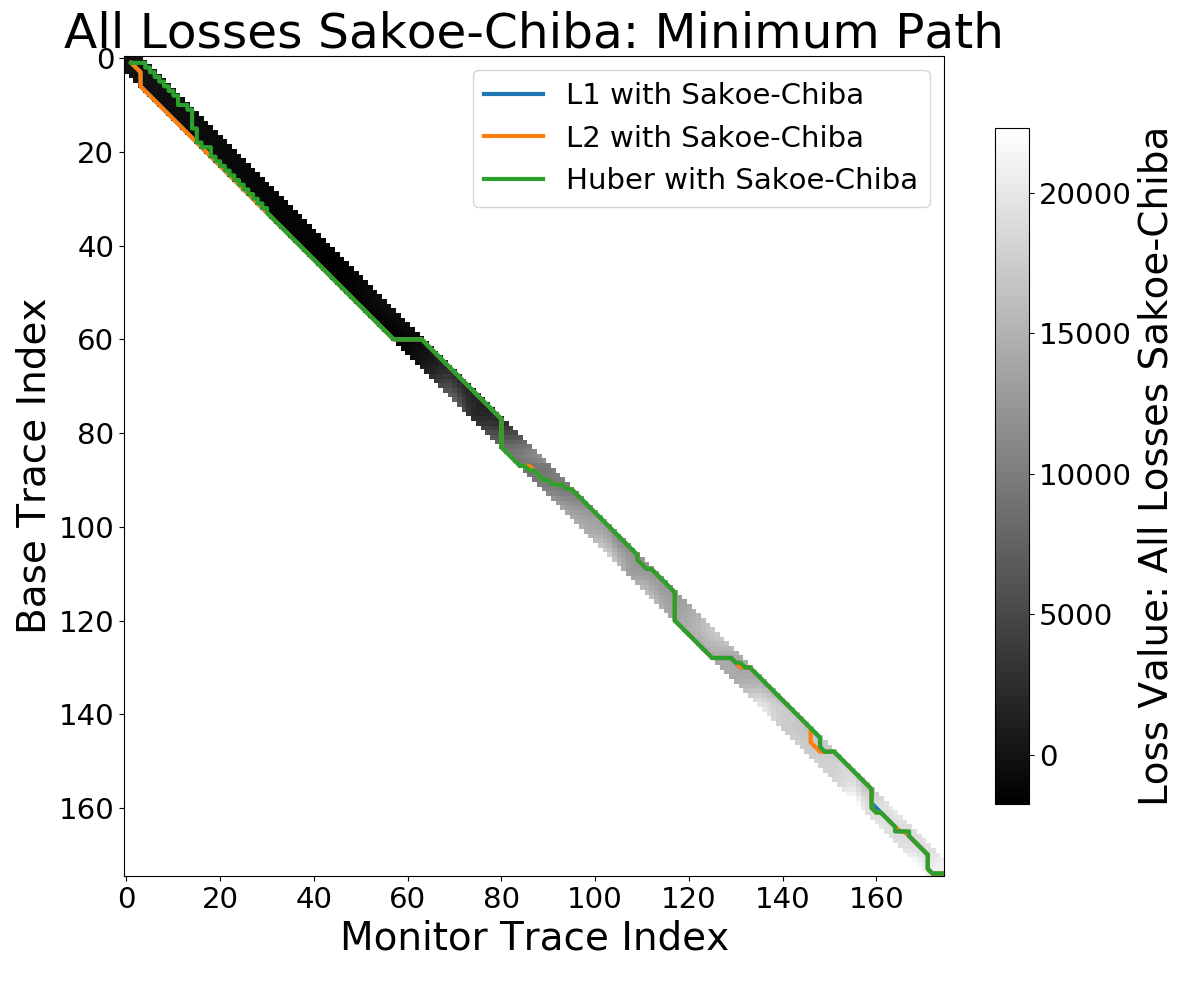
\includegraphics[width=.3\textwidth]{figures/minimum_path_all_losses_sakoe_chiba_.png} \label{fig:sakoe}
    }
    ~
    \subbottom[LB\_Envelope \citep{keogh2005exact}]{%
     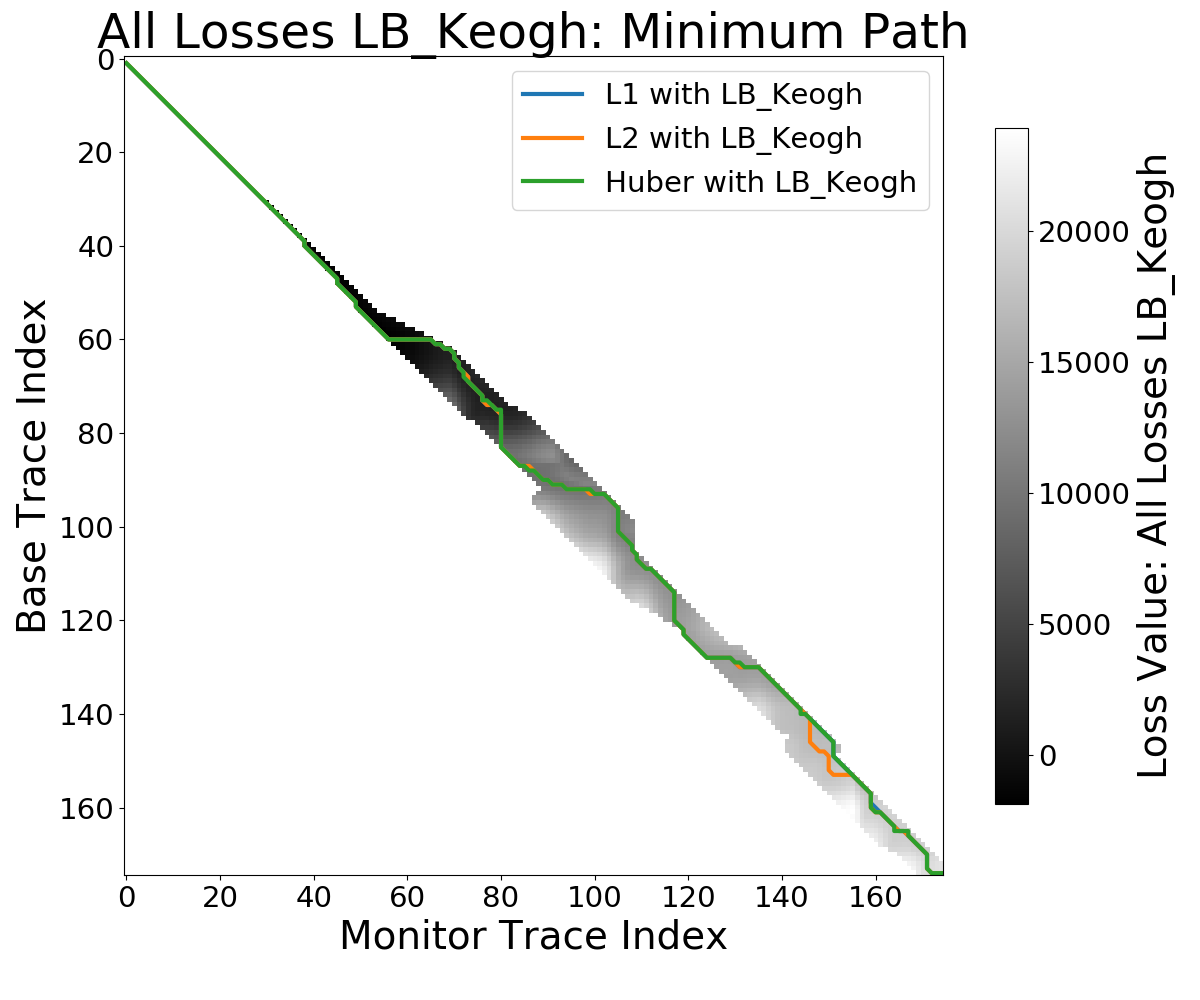
\includegraphics[width=.3\textwidth]{figures/minimum_path_all_losses_lb_keogh_.png}\label{fig:lbk}
    }
\caption{Minimum path for constraint masks for cumulative cost in \ac{dtw}.}
\label{fig:constraints}
\end{figure} 

Additionally, the search space on the cumulative distance matrix can be constrained to both increase performance and avoid non-optimal solutions. The different contraint strategies are presented in \cref{fig:constraints}. The Itakura parallelogram \citep{Itakura1975} in \cref{fig:itakura} describes a parallelogram that that has the largest width agress the diagonal of the matrix, providing the most flexibility for the \ac{dtw} algorithm in the center parts of the seismic traces. The Sakoe-Chiba disc \citep{Sakoe1978} follows a different strategy, which provides a constant maximum warp path. This strategy in \cref{fig:sakoe} introduces a global maximum time shift. Contrary to these two global constraints, we introduce the LB\_Keogh constraint in the paper. This lower bounding method provides a mathematical lower bound for the \ac{dtw} algorithm. We use this lower bound to constrain the warp path, which provides larger variability to high amplitude areas, where cycle-skipping can occur, presented in \cref{fig:lbk}. 

% dramsch2018information
In \citet{dramsch2018information} I was able to transfer the insight from applying the LB\_Keogh constraint to \aclp{cnn}. \acp{cnn} apply a windowed convolution to the data it is provided with. 
% Recent advances in machine learning relies on convolutional deep neural networks. These are often trained on cropped image patches. Pertaining to non-stationary seismic signals this may introduce low frequency noise and non-generalizability.

% dramsch2019complex
% Deep learning has become an area of interest in most scientific areas, including physical sciences. Modern networks apply real-valued transformations on the data. Particularly, convolutions in convolutional neural networks discard phase information entirely. Many deterministic signals, such as seismic data or electrical signals, contain significant information in the phase of the signal. We explore complex-valued deep convolutional networks to leverage non-linear feature maps. Seismic data commonly has a lowcut filter applied, to attenuate noise from ocean waves and similar long wavelength contributions. Discarding the phase information leads to low-frequency aliasing analogous to the Nyquist-Shannon theorem for high frequencies. In non-stationary data, the phase content can stabilize training and improve the generalizability of neural networks. While it has been shown that phase content can be restored in deep neural networks, we show how including phase information in feature maps improves both training and inference from deterministic physical data. Furthermore, we show that the reduction of parameters in a complex network results in training on a smaller dataset without overfitting, in comparison to a real-valued network with the same performance.


% dramsch2018deep
% We explore propagation of seismic interpretation by deep learning in stacked 2D sections. We show the application of state-of-the-art image classification algorithms on seismic data. These algorithms were trained on big labeled photograph databases. We use transfer learning to benefit from pre-trained networks and evaluate their performance on seismic data.